\section{1174005 - Oniwaldus Bere Mali}
\subsection{Teori}
\begin{enumerate}

\item Sejarah dan Perkembangan
	\hfill\break
	Definisi kecerdasan buatan (AI) Kecerdasan buatan (Bahasa Inggris: kecerdasan buatan atau AI) didefinisikan sebagai kecerdasan entitas ilmiah. Sistem ini umumnya dianggap komputer. Kecerdasan dibuat dan ditempatkan di sebuah mesin (komputer) sehingga dapat berfungsi seperti manusia. Berbagai jenis bidang yang menggunakan kecerdasan buatan meliputi sistem pakar, permainan komputer (game), logika fuzzy, jaringan saraf tiruan, dan robotika. Banyak hal yang tampaknya sulit bagi kecerdasan manusia, tetapi bagi ilmu komputer, relatif tidak bermasalah. Misalnya: mengubah persamaan, memecahkan persamaan integral, melakukan catur atau backgammon. Di sisi lain, hal-hal yang tampaknya membutuhkan sedikit kecerdasan bagi orang masih sulit untuk diproses dalam pengolahan data. Misalnya: 1. kecerdasan: kemampuan untuk memperoleh dan menggunakan pengetahuan 2. atau kecerdasan yang diukur dengan tes kecerdasan. KONSEP DASAR KECERDASAN ARTIFICIAL INTELLIGENCE (AI) Kecerdasan buatan dapat didefinisikan sebagai cabang ilmu komputer yang mempelajari otomatisasi perilaku cerdas (intelligent). Kecerdasan buatan dapat membuat komputer berpikir. Kecerdasan buatan dapat meniru proses pembelajaran manusia sehingga informasi baru dapat diserap dan digunakan sebagai referensi untuk masa depan. Asumsi dasar: hipotesis yang berkaitan dengan sistem simbol fisik (PSSH): proses pemrosesan informasi dapat dianggap sebagai pemrosesan atau manipulasi simbol, di mana informasi. 2. dilambangkan dengan simbol. Hipotesis-hipotesis ini memunculkan apa yang disebut elaborasi simbolis (ditemukan oleh Newell dan Simon). Perbedaan antara kecerdasan buatan (komputer) dan kecerdasan alami (manusia): Kecerdasan buatan: · permanen · mudah diduplikasi dan disebarkan · bisa lebih murah daripada orang cerdas · konsisten dan lengkap · dapat didokumentasikan Kecerdasan alami: · Jadilah kreatif · 
	
	\item Kecerdasan buatan terbagi atas beberapa metode yaitu:
	\hfill\break
	Supervised learning, Unsupervised Learning, Klasifikasi, Regresi, Dataset, Trainingset dan juga Testingset.
	\begin{itemize}
		\item Supervised Learning
		\hfill\break
		Sebuah algoritma pembelajaran mesin yang dapat menerapkan informasi yang sudah ada dalam data dengan memberikan label tertentu, misalnya data yang telah diklasifikasikan sebelumnya (diarahkan). Algoritma ini mampu memberikan target untuk output yang dilakukan dengan membandingkan pengalaman belajar masa yang sudah lampau.
		\item Unsupervised Learning 
		\hfill\break
		Berbeda dengan Supervised Learning, Unsupervised Learning ialah sebuah pembelajaran mesin tanpa pengawasan adalah pembelajaran mesin yang digunakan pada data yang tidak memiliki informasi yang dapat diterapkan secara langsung (tidak diarahkan). Algoritma ini diharapkan dapat menemukan struktur tersembunyi dalam data yang tidak berlabel.
		\item Klasifikasi
		\hfill\break
		Klasifikasi adalah sampel milik dua kelas atau lebih dan ingin belajar dari data yang sudah diberi label cara memprediksi kelas data yang tidak berlabel. Contoh masalah klasifikasi adalah pengenalan digit tulisan tangan, di mana tujuannya adalah untuk menetapkan masing-masing vektor input ke salah satu dari sejumlah kategori diskrit. 
		\item Regresi
		\hfill\break
		Regrasi ialah sebuah metode untuk mengembangkan model (persamaan) yang menjelaskan hubungan antara beberapa variabel. Output dari analisis regresi adalah persamaan regresi. Dalam model regresi variabel dibagi menjadi dua bagian, yaitu variabel respon atau yang biasa juga disebut variabel dependen dan variabel explanatory atau juga biasa disebut variabel prediktor atau disebut juga variabel independen.
		\item Data set
		\hfill\break
		Dataset adalah sebuah kumpulan data atau objek dan bagaimana relasi dalam memori. Struktur Dataset mirip dengan data di dalam database. Dataset berisi koleksi dari datatable maupun data relasi.
		\item Training Set
		\hfill\break
		Training set ialah bagian dari dataset yang berfungsi untuk membuat prediksi atau mengatur fungsi dari algoritma-algoritma yang ada. Fungsi nya yang lain juga ada sesuai tujuannya masing-masing. Trainingset memberikan instruksi melalui algoritma sehingga mesin dapat mengerti dan membuat kolerasi sendiri.		
		\item Testing Set
		\hfill\break
		Sama seperti training set, testing set juga bagian dari dataset yang berfungsi menguji untuk melihat akurasinya, atau bisa juga untuk melihat suatu kinerja atau performa.
	\end{itemize}
\end{enumerate}
\end{enumerate}
\subsection{Praktek}
\begin{enumerate}
	\item Instalasi Library scikit dari Anaconda, mencoba kompilasi dan uji coba ambil contoh kode dan lihat variabel explorer
	\hfill\break
	\begin{figure}[H]
		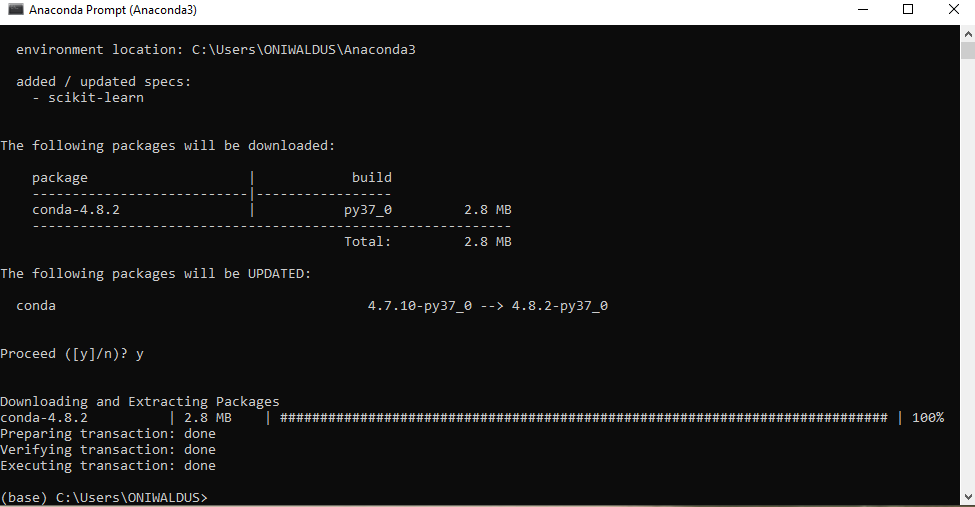
\includegraphics[width=4cm]{figures/1174005/tugas1/materi/1.PNG}
		\centering
		\caption{Instalasi Library Scikit Learn}
	\end{figure}
	\begin{figure}[H]
		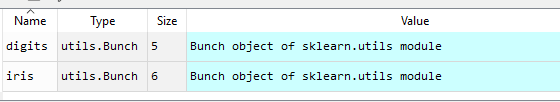
\includegraphics[width=4cm]{figures/1174005/tugas1/materi/2.PNG}
		\centering
		\caption{Isi Variabel Explorer}
	\end{figure}
	\item Uji coba loading an example dataset
	\hfill\break
	\lstinputlisting[firstline=7, lastline=12]{src/1174005/1174005.py}
	\item Uji coba Learning dan predicting
	\hfill\break
	\lstinputlisting[firstline=15, lastline=18]{src/1174005/1174005.py}
	\item Uji coba Model Persistence
	\hfill\break
	\lstinputlisting[firstline=21, lastline=37]{src/1174005/1174005.py}
	\item Uji coba Conventions
	\hfill\break
	\lstinputlisting[firstline=40, lastline=52]{src/1174005/1174005.py}
\end{enumerate}
\subsection{Penanganan Error}
\begin{enumerate}
	\item ScreenShoot Error
	\begin{figure}[H]
		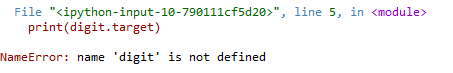
\includegraphics[width=4cm]{figures/1174005/tugas1/error/3.PNG}
		\centering
		\caption{NameError: name 'digit' is not defined}
	\end{figure}
	\begin{figure}[H]
		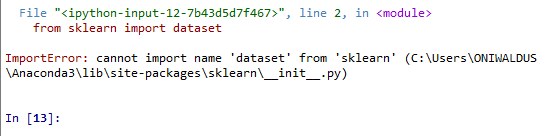
\includegraphics[width=4cm]{figures/1174005/tugas1/error/4.PNG}
		\centering
		\caption{Import Error}
	\end{figure}
	\item Tuliskan Kode Error dan Jenis Error
	\begin{itemize}
		\item NameError: name 'digit' is not defined
		\item Import Error
	\end{itemize}
	\item Cara Penangan Error
	\begin{itemize}
		\item NameError: name 'digit' is not defined
		\hfill\break
		Error terdapat pada digit dan seharusnya digids
		\item Import Error
		\hfill\break
		Error terdapat typo pada dataset, seharusnya datasets
	\end{itemize}
\end{enumerate}
\subsection{Bukti Tidak Plagiat}
\begin{figure}[H]
	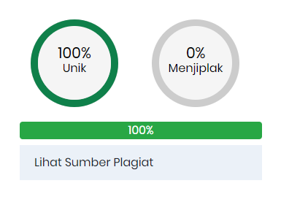
\includegraphics[width=4cm]{figures/1174005/tugas1/plagiat/5.PNG}
	\centering
	\caption{Bukti Tidak Melakukan Plagiat Chapter 1}
\end{figure}